\documentclass{sig-alternate}
\usepackage{color}
\usepackage[colorinlistoftodos]{todonotes}
\usepackage{amssymb}
\usepackage{upgreek}
\begin{document}
\conferenceinfo{UMM CSci Senior Seminar Conference, December 2014}{Morris, MN}

\title{Gait Recognition in Mobile Security}

\numberofauthors{1}

\author{
\alignauthor
Chase R. Ottomoeller\\
	\affaddr{Division of Science and Mathematics}\\
	\affaddr{University of Minnesota, Morris}\\
	\affaddr{Morris, Minnesota, USA 56267}\\
	\email{ottom005@morris.umn.edu}
}

\maketitle
%----------------------------------------------------------------------------------------------------------------------%
\begin{abstract}
This paper discusses a new form of mobile security not just emphasizing security, but also usability. Having a form of security of a mobile device that is unobtrusive can make that device easier and a less of a hassle to use. This paper will discuss using built in accelerometers in smart phones as a way to collect biometric data. In this case the biometric data is a persons gait or walking pattern. This increases the security of the device by allowing the authentication to not be something you have or something you know, but something you are. There are two example that this paper will compare showing two forms of gait analysis. 
\end{abstract}

\keywords{mobile security, gait recognition, biometrics, accelerometer}
%----------------------------------------------------------------------------------------------------------------------%
\section{Introduction}
	As computational power in computers increases, the security risks grow higher for forms of authentication. One growing concern is security in mobile devices such as smart phones. Smart phones are also becoming increasingly more powerful, which results in more personal data being stored on the device. This means security for smart phones will become more important as time goes on. Currently security mainly consists of: pin, password, swipe lock, fingerprint. These forms are either something a person has(fingerprint) or something a person knows(password). They all also require a physical action to unlock the phone. A new form of mobile security involves a persons gait making it an unobtrusive form of security. This means that the built in accelerometer in the smart phone will analyze a persons walking pattern. If the phone tell that the current user should have access the phone will be unlocked, otherwise it will switch to the normal pin password. This will increase the security of the mobile device because the form of unlocking the device is now something you are and not something someone else can take form you. 
	This paper will analyse two different approaches for gait extraction/analysis. Each paper uses a general format format of analysing the data which includes: Preprocessing, Feature Extraction, and Gait Analysis. Preprocessing is the process of capturing biometric data. Feature extraction is taking the raw biometric data and locating distinctive characteristics. Gait Analysis is taking the feature extracted data,and running algorithm on it which will return a positive or negative result. Though each paper follows this general outline, they did each step in a different way.

%\begin{figure}
%\centering
%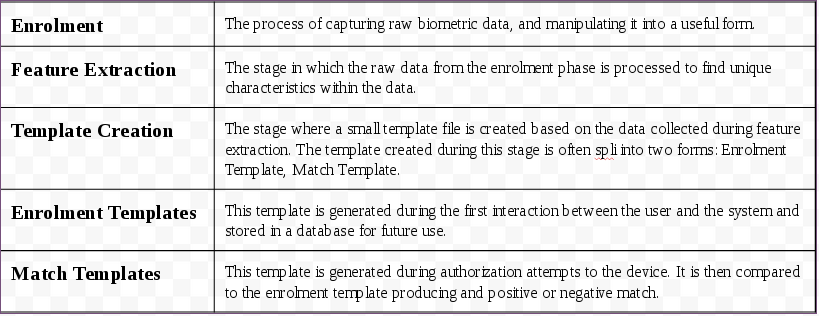
\psfig{file=chart3.png,width =3in}
%\caption{}
%\label{fig:Steps}
%\end{figure}

%I plan to use the following sources:
%\begin{itemize}
%\item one~\cite{Sujithra:2012}
%\item two~\cite{Muaaz:2013}
%\item three~\cite{Lu:2014}
%\end{itemize}
%----------------------------------------------------------------------------------------------------------------------%
\section{Background}
	Biometrics is used as a new form of security that provides unique identification to a mobile user. Now, instead of relying on a password of physical key, a person can gain access to their device by a physical trait specific to them. Some examples of biometric traits are: finger prints, facial features, eye, voice, hand, DNA, gait. In this paper I will focus on the gait recognition. The term gait refers to the walking pattern of a person. A persons walking pattern is cyclic in nature and may be composed of many gait cycles, where each gait cycle consists of at least two steps.~\cite{Sujithra:2012} 
	There are three types of biometric gait recognition: machine vision based, floor sensor based, and wearable sensor based. With mobile devices becoming more and more equipped with an array of sensors, the technique most suited for mobile devices is a wearable sensor based, using the mobiles devices built-in accelerometer. Data collected from the accelerometer will be processed in a set of operations later described. 
	In the next sections I will be comparing two approaches that use accelerometers from a mobile device such as a smart phone. The primary way in which these two approaches differ is the placement of the mobile device on the body. One approach has the smart phone in a fixed location on the waist. I will refer to this method as the \textit{fixed} method. The other method has the smart phone in a more natural position on the body such as in a pocket. This method will be referred to as the \textit{unfixed} method. Though both papers use the general approach shown in figure ~\ref{fig:Paper1Summary} I will be simplifying them into three categories: Pre-Processing, Feature Extraction, and Gait Analysis. 
%----------------------------------------------------------------------------------------------------------------------%
\section{Preprocessing} 
Once data is gathered it needs to preprocesed into a usable form. For this paper a usable form is modified data that has been separated into frames. A frame is equally separated parts of data for feature extraction and classification. With two methods (fixed and unfixed), separating the data into modified frames was done differently. The fixed phone method used a strict test case that was modified using Linear Interpolation and Zero Normalization. The unfixed phone method used Framing and Projection. Framing separated the data into frames. These frames were then modified by using Projection. In the following sections I will explain the fixed and unfixed methods as well as compare them. 
		%\\\\\\\\\\\\\\\\\\\\\\\\\\\\\\\\\\\\\\\\\\\\\\\\\\\\\\\\\\\\\\\\\\\\\\\\\\\\\\\\\\\\\\\\\\\\\\\\\\\\\\\\%
\subsection{Fixed Method Preprocessing}	
	With the phone on the waist in a fixed position, uniform sets of data called walks were used. In this case one walk is represented by walking a measured distance down a hallway. The experiment was done is such a way that one set of data contained two "walks", or in other words, one set of data was walking a hallway; Once down and once back. After extracted, this data is modified to further extract features. These modifications include linear interpolation and zero normalization. 
			%+++++++++++++++++++++++++++++++++++++++++++++++++++++++++++++++++++++++++++++++++++%
\subsubsection{Interpolation} 
	Once the walks are separated from the initial data, they have to be formed into equal intervals. This is done by applying \textit{Linear Interpolation}, which can reshape the data  into equal intervals. In order to not loose data during this change up-sampling is applied. Up-sampling avoids data loss by producing ``an approximation of the sequence that would have been obtained by sampling the signal at a higher rate''~\cite{wiki1:2014}. Once the data has been reshaped, the acceleration measurements have to be adjusted. 
			%+++++++++++++++++++++++++++++++++++++++++++++++++++++++++++++++++++++++++++++++++++%
\subsubsection{Zero Normalization}
	The PMDs accelerometer being used measures 3 axis(X, Y, Z). the only axis needed, and the only axis affected by gravity is the X axis. Since the acceleration for the Y and Z axis are not stable over time, and they are not affected by earth's gravity, the acceleration data for the Y and Z axis have to be \textit{zero normalized}. In other words the data for the Y and Z axis have to be set to zero. This is done by simply subtracting their total acceleration from there average acceleration. An overview of the stages explained above are shown in figure ~\ref{fig:firstStep}.


		%\\\\\\\\\\\\\\\\\\\\\\\\\\\\\\\\\\\\\\\\\\\\\\\\\\\\\\\\\\\\\\\\\\\\\\\\\\\\\\\\\\\\\\\\\\\\\\\\\\\\\\\\%
\subsection{Un-fixed Method Preprocessing}{
	The previous method used a phone in a fixed location. This method tries to expand on this with a phone in a unfixed location, such as a pocket. Also, this method is less strict. It does no use a set length, such as a hallway, to mark each walk. Instead this method uses a processes called \textit{Framing}. Once the data is segmented into frames it is then projected onto a global coordinate system through a process know as \textit{Projection}.
	}
			%+++++++++++++++++++++++++++++++++++++++++++++++++++++++++++++++++++++++++++++++++++%
\subsubsection{Framing}{
 During Framing, sensor data is segmented into uniform frames for feature extraction and feature classification. Unlike the data for the fixed method, this data is segmented into 512 equal length samples. This is done by taking a sample every 5.12 seconds. They state the reason for 512 samples was "to balance between estimation accuracy and latency. Also, not all frames move onto feature extraction. Frames that are below a chosen threshold, representing no movement, are dropped. 
 }
 			%+++++++++++++++++++++++++++++++++++++++++++++++++++++++++++++++++++++++++++++++++++%
\subsubsection{Projection}{
Each sample within a given frame contains an X, Y and Z coordinate. Each coordinate is then projected into a vertical and horizontal variable. Once each sample is projected, the direction of gravity is determined by using a mean filter. Unlike the previous example, this process doesn't assume a fixed location or orientation of the mobile device. If there is a significant change in the gravity variable then the orientation of the device has changed. This means the corresponding frame will be dropped and the horizontal and vertical axes will be adjusted accordingly. 
}

Both the fixed and unfixed method split the data into equal intervals and then modify the data so that it is able to be worked with. The reason for the differences between stems from the differences in phone placement. The data collected in the fixed method is already more organized than the data from the unfixed method. This is because the unfixed method has to worry about all axis as well as organizing the data into neater parts. If the fixed method were to be implemented in more of a real life scenario then these methods become even more similar. 
%----------------------------------------------------------------------------------------------------------------------%

\section{Feature Extraction}
	\textit{Feature Extraction} is extracting a set of data from a given frame to detect patterns of walking. Another way to define feature extraction is the process of extracting gait cycles from the data. 
		%\\\\\\\\\\\\\\\\\\\\\\\\\\\\\\\\\\\\\\\\\\\\\\\\\\\\\\\\\\\\\\\\\\\\\\\\\\\\\\\\\\\\\\\\\\\\\\\\\\\\\\\\%
\subsection{Fixed Method Feature Extraction}
	The fixed method in order uses the following steps as seen in figure~\ref{fig:AccelChart}: Cycle length estimation, Cycle detection, Cycle length normalization, Omitting unusual cycles.
			%+++++++++++++++++++++++++++++++++++++++++++++++++++++++++++++++++++++++++++++++++++%
\subsubsection{Cycle Length Estimation}
Once the raw gait data is preprocessed, the next step is extracting the biometric gait cycles. The first step in extraction is to be able to automatically detect gait cycles in the walk. This detection is done by estimating the cycle length, which is simply computing minimum salience vector. There is a minimum salience vector for each data point for a given walk. Each minimum salience vector is computed by counting the data values that are between that current data value and the following smaller value in the walk vector. If the current salience vector is greater than the minimal peak distance or height, it is a cycle start. This same process is used to determine the maximum peak and distance as well.
			%+++++++++++++++++++++++++++++++++++++++++++++++++++++++++++++++++++++++++++++++++++%
\subsubsection{Cycle Detection}
Once both minimum and maximum salience vectors are computed so they can be used to detect individual cycles. A good example can be seen in figure ~\ref{fig:TD1}. In this figure the minimum salience vectors are seen in blue and the accelerometer data is seen in red. We can easily see where the start of each cycle is based on the minimum salience vector. Maximum salience vectors are also computed to help determine the exact minima.
			%+++++++++++++++++++++++++++++++++++++++++++++++++++++++++++++++++++++++++++++++++++%
\subsubsection{Cycle Length Normalization}
Using linear interpolation again, the determined cycles are normalized to a set length. These set lengths are later required in the Euclidean distance which requires vectors of the same length.
			%+++++++++++++++++++++++++++++++++++++++++++++++++++++++++++++++++++++++++++++++++++%
\subsubsection{Omitting Unusual Cycles}
Some cycles compared to the majority are considered unusual. These could be caused by any motion or non-motion that isn't walking. This is done by ``computing the distance using \textit{Dynamic Time Warping} (DTW).''~\cite{Muaaz:2013} Dynamic time warping is ``an algorithm for measuring similarity between two temporal sequences which may vary in time or speed.''~\cite{wiki2:2014}This means that cycles with a distance of half or more of the other cycles will be removed.

		%\\\\\\\\\\\\\\\\\\\\\\\\\\\\\\\\\\\\\\\\\\\\\\\\\\\\\\\\\\\\\\\\\\\\\\\\\\\\\\\\\\\\\\\\\\\\\\\\\\\\\\\\%
\subsection{Unfixed Method Feature Extraction}
	A different form of extraction used by ~\cite{Lu:2014} uses a combination of time-domain, frequency-domain, and auto-correlation features. This example also did feature extraction in two stages: calculating the set of features for walking and calculating more precise gait features. 
			%+++++++++++++++++++++++++++++++++++++++++++++++++++++++++++++++++++++++++++++++++++%
\subsubsection{Feature Extraction I}
	The first stage of the feature extraction is used to tell whether or not the data represents walking data. This is done to rule out the times when the mobile device is not collecting the right data. For example if the mobile device was collecting data when it was in a car going down the road, that data shouldn't be used because it isn't gait data. This also holds true for collecting data on someone who is standing still. The data collected wouldn't represent the data needed for a biometric. Telling whether the data collected is of someone walking is done by collecting vertical and horizontal features to produce motion patters. Six time-domain features are used for both directions. These six feature are :mean, variance, skewness, kurtosis, energy, mean-crossing rate. All these features are based on spectrum analysis. In other words, doing ``different activities have different energy distributions over the frequency spectrum.''~\cite{Lu:2014} Walking can be measured around 1-2Hz while driving in a car will output a higher frequency band. Based on these frequency levels the data is put into one of three classes: walking, non-walking and motion(high frequency movement such as a in a vehicle or running).~\cite{Muaaz:2013}
			%+++++++++++++++++++++++++++++++++++++++++++++++++++++++++++++++++++++++++++++++++++%
\subsubsection{Walking Detection}
	Using data from feature extraction I, classification can be done using a decision tree.There are three activities that the data can be classified as: walking, non-walking, and random movements. Non-walking motion is running, biking, or moving in a vehicle. Random motion is a motion such as turning or skipping. A Markov Model smoother is applied to the new set of data to get rid of any outliers. 
			%+++++++++++++++++++++++++++++++++++++++++++++++++++++++++++++++++++++++++++++++++++%
\subsubsection{Feature Extraction II}{
	Feature extraction II is done once the data collected is determined to be gait data. In this stage more relevant features are extracted for analysis. The first analysis to be done is the Compressed sub-band cepstral coefficients(CSCC). This is done in the following three steps. First, the energy spectrum is computed using the FFT spectrum. The Fast Fourier Transform(FFT) is an alogorithm that computes the Discrete Fourieer Transform(DFT) and its inverse. The study maps the energy spectrum into 26 bands using triangular overlapping bands and sum up the energy in each band. The processing then takes the discrete cosine transform of the sub-band energy to form a 12-dimension vector representation. This in all summarizes the fundamental frequency of the movements and the higher frequency vibrations in the data.~\cite{Sujithra:2012}
}

	Both of these methods of feature extraction try to determine what parts of the data represent a walk cycle. The fixed method is simpler because it doesn't have to worry about different variables affecting the data. Though this method is simpler, it has the stipulation of the mobile device being clipped to your waste. The non-fixed method has to worry about more variables affecting the data, but implements a real life situation of just having the mobile device in a pocket.
	
	
%----------------------------------------------------------------------------------------------------------------------%
\section{Gait Classification}
	This last step is taking the extracted features and verifying that those features match a stored set of features; the stored set of features being the users. The fixed method uses Support Vector Machines(SVM's). The basic idea of SVM's is taking dimensional data and separating it into two classes. This involves the use of a Gaussian kernel defined in the following section. The unfixed method uses a Gaussian Mixture Model - Universal Background Model(GMM-UBM) framework to verify a individuals gait. The basic idea with this technique is with scoring. Verification of a users identity is done by comparing the likelihood score from a users gait pattern to the universal back ground model. The universal back ground model represents human gait patterns in general.


		%\\\\\\\\\\\\\\\\\\\\\\\\\\\\\\\\\\\\\\\\\\\\\\\\\\\\\\\\\\\\\\\\\\\\\\\\\\\\\\\\\\\\\\\\\\\\\\\\\\\\\\\\%
\subsection{Template-based classification}
	The template-based classification uses the same approach for gait extraction as shown in~\ref{fig:SecondStep} with one extra step added show in \ref{fig:AddedStep}. Before the Cycle Length Estimation module is Piecewise Linear Approximation(PLA). A Piecewise Linear Function(PLF) is used for the PLA. A PLF is a function composed of straight-line sections connecting points on a graph. So, a PLA is an approximation of a function connecting significant points on the curve with straight-line sections. The approach used to produce the PLA representations is the
Sliding Window And Bottom-up(SWAB). Once the unusual cycles are omitted, the best cycle is picked. The best cycle is determined by having the lowest DTW 
%\todo[inline]{This section will be redone}
One the best cycle is foundA the remaining cycles are called probe cycles. These two sets of cycles are compared using the DTW distance to compute the genuine and impostor class. The DTW of each cycle is computed and majority voting takes place. If 50\% or more of the comparisons returns and accept then the cycle in a genuine, otherwise it's rejected as an imposter. 

		%\\\\\\\\\\\\\\\\\\\\\\\\\\\\\\\\\\\\\\\\\\\\\\\\\\\\\\\\\\\\\\\\\\\\\\\\\\\\\\\\\\\\\\\\\\\\\\\\\\\\\\\\%
\subsection{Fixed Method Gait Classification}
	SVMs are another way to classify gait data. SVMs are often used for biometric recognition, where imposter and genuine data have to be determined. First the SVM finds a \textit{hyperplane}. A hyperplane is a subspace that is one dimension less than its ``ambient space". For example, there could be a set of data represented by 3 axis (X,Y,Z). The hyperplane would be the same data plotted on a 2 axis space. So, the SVM will take the data, and find a hyperplane that linearly separates \begin{math}\mathcal{D} \end{math} dimensional data into two classes. The dimensional data has to be linearly separable for the SVM to work. Since the gait data isn't linearly separable, a ``kernel induced feature space''~\cite{Muaaz:2013} is introduced in the SVM. A kernel function maps non linearly separable data to a high dimensional space. Once mapped to a high dimensional space the data is linearly separable and therefore can be used by the SVM to find a hyperplane. This means that depending on the kernel function you use, the better classification accuracy it will produce. 
% Reword this to get rid of euclidean distance.	
%	Another more commonly used kernel function is the Gaussian kernel, which uses the Euclidean distance. Since the Euclidean distance restricts to only using fixed length cycles, 
There are kernel functions that would require the use of fixed length gait cycles. Since gait cycles are not usually of a fixed length, a different kernel is used. By using the DTW distance, the problem of fix-length input feature vectors can be solved as well as more accurate finding of similarity in the data. Two different approaches using SVM and DTW can be used to classify gait cycles:Pre-computed data matrix, and Pre-computed kernel. ~\ref{fig:TrainingData}

			%+++++++++++++++++++++++++++++++++++++++++++++++++++++++++++++++++++++++++++++++++++%
\subsubsection{Pre-computed data matrix}
	Gait cycles are represented by the DTW distance. The DTW distance is the distance between two gait cycles. The benefit of the DTW distance is that gait cycles with different length can be found. A DTW matrix is then computed by taking the sample DTW distance and compared to all other samples. This matrix is needed as an input for the SVM.
	
			%+++++++++++++++++++++++++++++++++++++++++++++++++++++++++++++++++++++++++++++++++++%
\subsubsection{Pre-computed Kernel}
Using GDTW kernel equation ~\ref{eq:KF3} as the kernel matrix also allows to classify the gait data. Though this kernel matrix is a symmetric matrix, it is not guaranteed that it has all positive eigenvalues. 

\begin{equation} \label{eq:KF3}
K(x,z)=exp(-\gamma \parallel DTW(x,z) \parallel ^2)
\end{equation}

		%\\\\\\\\\\\\\\\\\\\\\\\\\\\\\\\\\\\\\\\\\\\\\\\\\\\\\\\\\\\\\\\\\\\\\\\\\\\\\\\\\\\\\\\\\\\\\\\\\\\\\\\\%
\subsection{Unfixed Method Gait Classification}
The framework used for classifying gait cycles is a Gaussian Mixture Model-Universal Background (GMM-UBM). The algorithm can be split into three primary sections: UBM training, user gait model genertion, runtime inference and adaptation. 

	 The UBM is a large Universal background GMM that is trained from a large source of data. This means a UBM represents the general walk pattern of humans. The UBM is defined as 
\begin{math} \lambda \end{math} (\begin{math} \omega \end{math},
\begin{math} \upmu \end{math},
\begin{math} \Sigma \end{math}) where
\begin{math} \omega \end{math} represents the mixture weight, \begin{math} \upmu \end{math} represents the mean, and \begin{math} \Sigma \end{math} represents the covariance matrix. In other words \begin{math} \omega \end{math} is the prior distribution of waling patterns while \begin{math} \upmu \end{math} and \begin{math} \Sigma \end{math} are different walking patterns given by the population in different conditions. For efficiency the \textit{covariance matrix} is used. A covariance matrix ``generalizes the notion of variance to multiple dimensions.'' Also, to avoid over fitting the training data, a standard expectation maximization (EM) algorithm is applied. The EM is what trains the UBM models. For example, if given a collection of training vectors, the EM estimates the parameters to most likely to occur. The EM algorithm does this through iteration. Each time the algorithm iterates it refines the GMM parameters, increasing the likelihood of the estimated model for the given feature vectors.
%maybe provide an example?????
%----------------------------------------------------------------------------------------------------------------------%
%\section{Experiment Results}
%\subsubsection{Paper 1(title place holder)}
%\subsubsection{Paper 2(title place holder)}


%----------------------------------------------------------------------------------------------------------------------%
\section{Putting it all Together}
I have compared two forms of using built gait as a form of mobile security. One experiment used a fixed location for the device while the other used multiple locations. Both use different methods of extracting the gait data as well as well as analyzing the data, but each method works. Both of these experiments are not perfect yet but they both show promise in using walking patterns as a form of mobile security. With more sampling/testing as well as improving efficiency with algorithms will improve these mobile security methods and show potential to become implemented in a large scale. 
%----------------------------------------------------------------------------------------------------------------------%

\section{Acknowledgments}
% The following two commands are all you need to
% produce the bibliography for the citations in your paper.
\bibliographystyle{abbrv}
% annotated_bibliography.bib is the name of the BibTex file containing 
% all the bibliography entries for this example. Note that you *don't* include the .bib ending
% in the \bibliography command.
%----------------------------------------------------------------------------------------------------------------------%
\bibliography{paper}  

% You must have a ".bib" file and remember to run:
%     pdflatex bibtex pdflatex pdflatex
% in order to see all the citation references correctly.

%@@@@@@@@@@@@@@@@@@@@@@@@@@@@@@@@@@@@@@@@@@@@@@@@%
\begin{figure}
\centering
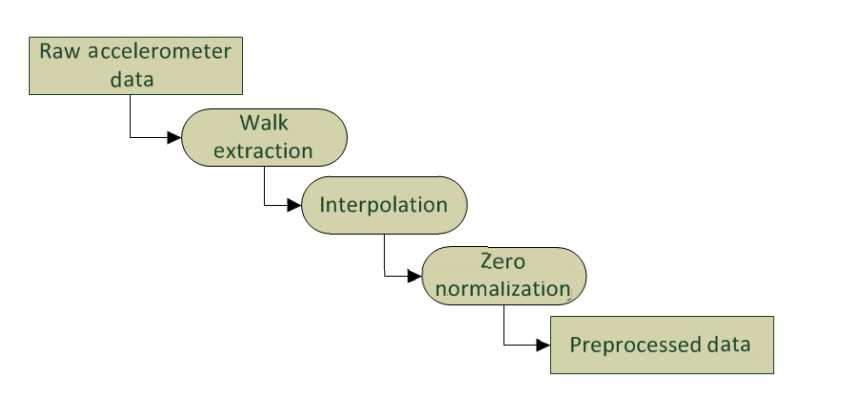
\psfig{file=chart1.png,width =3in}
\caption{Preprocessing Step}
\label{fig:firstStep}
\end{figure}

%@@@@@@@@@@@@@@@@@@@@@@@@@@@@@@@@@@@@@@@@@@@@@@@@%
\begin{figure*}
\centering
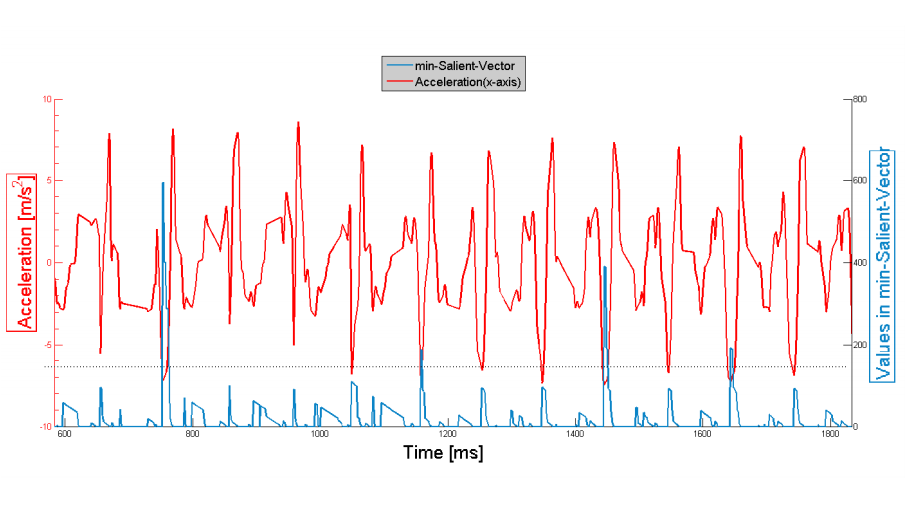
\psfig{file=svector.png,width =5.3in}
\caption{Minimum Salient Vectors}
\label{fig:AccelChart}
\end{figure*}

%@@@@@@@@@@@@@@@@@@@@@@@@@@@@@@@@@@@@@@@@@@@@@@@@%
\begin{figure}
\centering
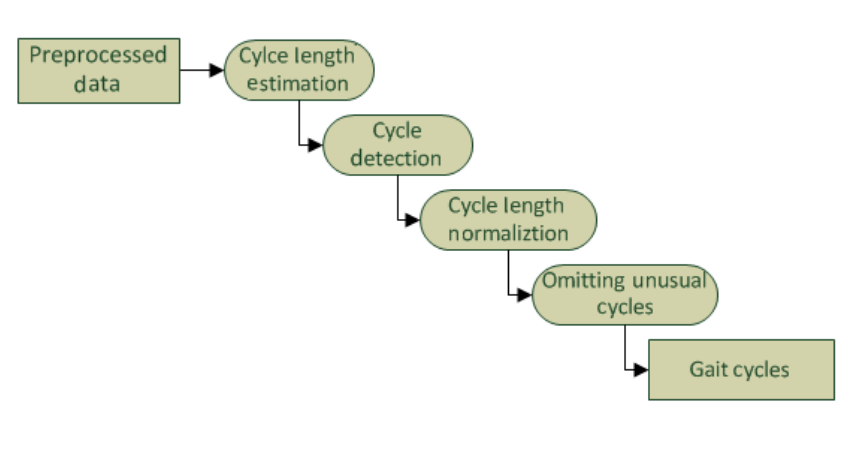
\psfig{file=chart2.png,width =3in}
\caption{Feature Extraction}
\label{fig:SecondStep}
\end{figure}

%@@@@@@@@@@@@@@@@@@@@@@@@@@@@@@@@@@@@@@@@@@@@@@@@%
\begin{figure}
\centering
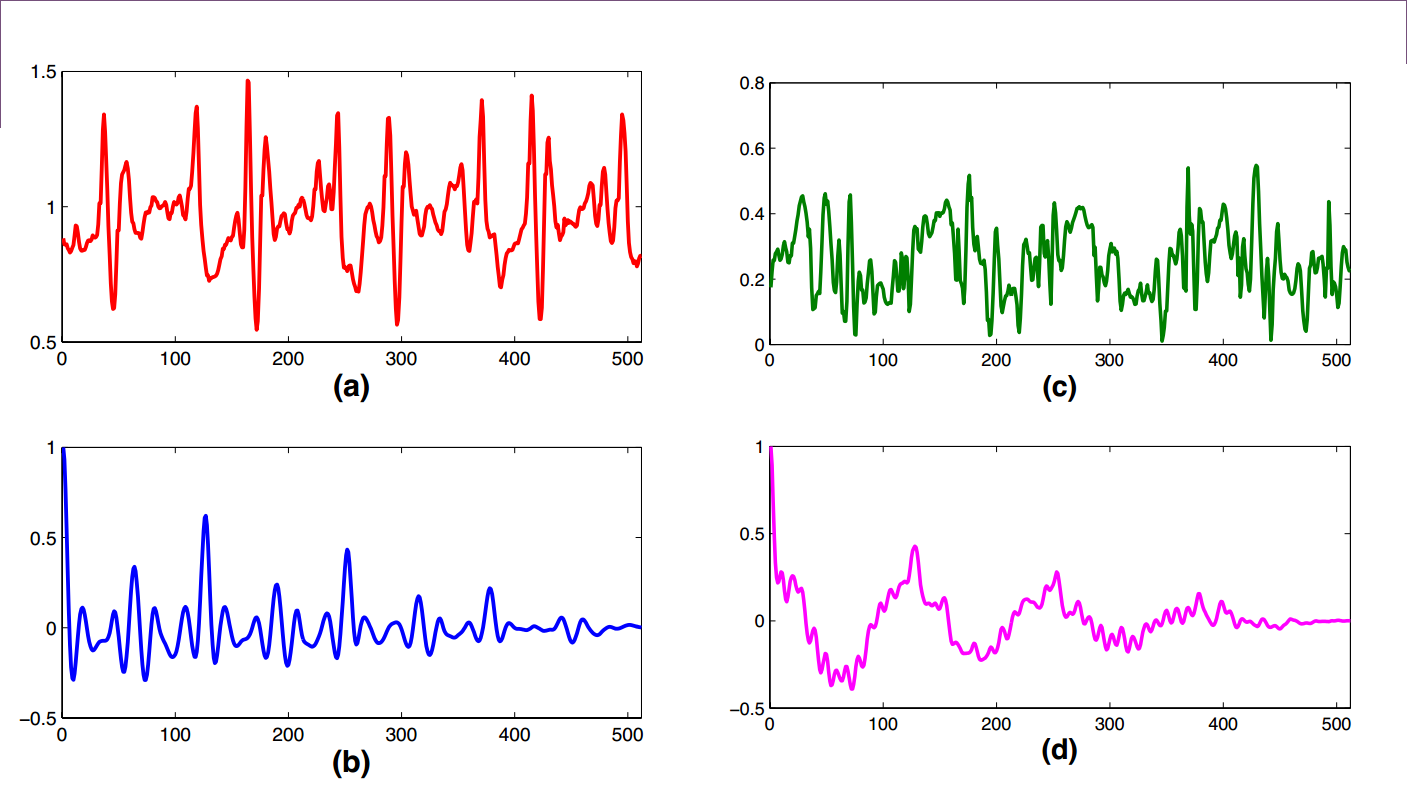
\psfig{file=abcd.png,width =3in}
\caption{(a) projected vertical component. (b) normalized autocorrelation of the vertical component. (c) projected horizontal component. (d) normalized autocorrelation of the horizontal component}
\label{fig:TD1}
\end{figure}

%@@@@@@@@@@@@@@@@@@@@@@@@@@@@@@@@@@@@@@@@@@@@@@@@%
\begin{figure}
\centering
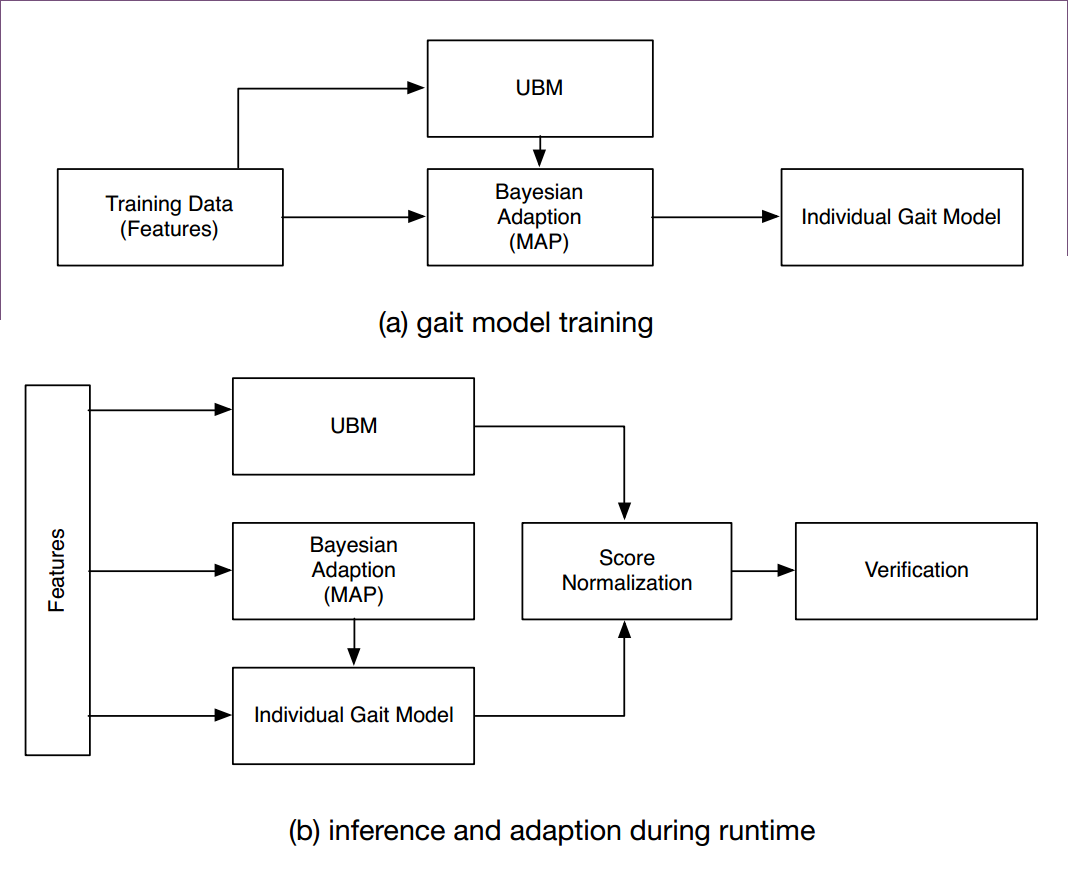
\psfig{file=FESP.png,width =3in}
\caption{Algorithm work-flow for (a) generate user gait model by MAP adaptation (b) runtime inference and Individual model adaptation}
\label{fig:TD2}
\end{figure}

%@@@@@@@@@@@@@@@@@@@@@@@@@@@@@@@@@@@@@@@@@@@@@@@@%
\begin{figure}
\centering
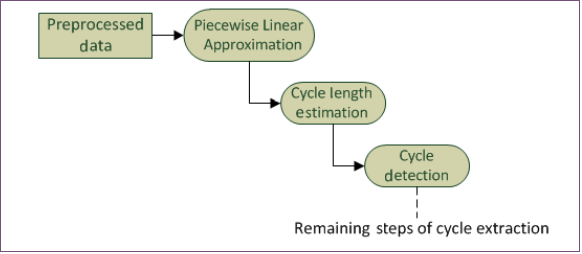
\psfig{file=PreprocessedData.png,width =3in}
\caption{Gait cycle extraction steps with Piecewise Linear Approximation(PLA)}
\label{fig:AddedStep}
\end{figure}

%@@@@@@@@@@@@@@@@@@@@@@@@@@@@@@@@@@@@@@@@@@@@@@@@%
\begin{figure}
\centering
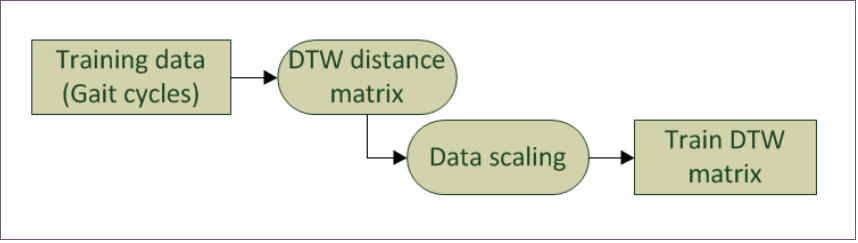
\psfig{file=TrainingData.png,width =3in}
\caption{Preparing data for SVM)}
\label{fig:TrainingData}
\end{figure}

%@@@@@@@@@@@@@@@@@@@@@@@@@@@@@@@@@@@@@@@@@@@@@@@@%
\begin{figure}
\centering
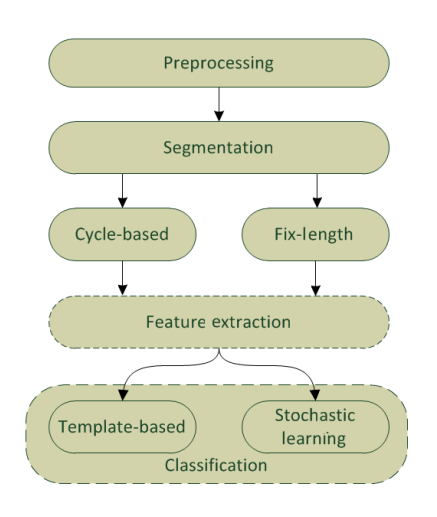
\psfig{file=sumary1.png,height =2.5in, width =2in}
\caption{Algorithm Overview}
\label{fig:Paper1Summary}
\end{figure}

%@@@@@@@@@@@@@@@@@@@@@@@@@@@@@@@@@@@@@@@@@@@@@@@@%
\begin{figure*}
\centering
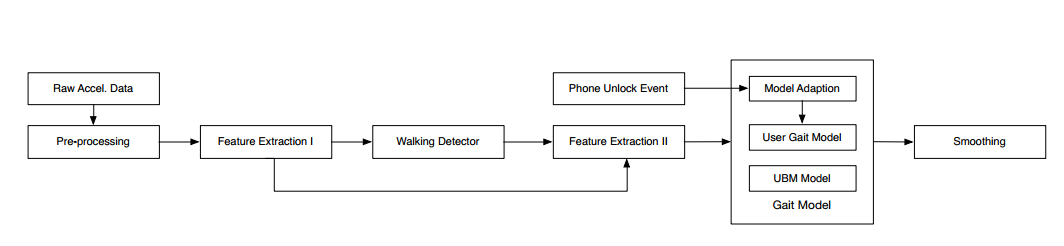
\psfig{file=sumary2.png,width =5.3in}
\caption{Algorithm Overview}
\label{fig:Paper2Summary}
\end{figure*}

%
%\begin{displaymath}
%K : X \times X \rightarrow \mathbb{R}, \forall \{x,z\} \in X
%\label{eq:KF1} 
%\end{displaymath}
%
%\begin{displaymath}
%K(x,z)=< \phi (x).\phi(z) > 
%\label{eq:KF2}
%\end{displaymath}

\end{document}



